\documentclass[12pt, a4paper]{report}

\usepackage{amsmath,amsthm,amssymb}
\usepackage{mathtext}
\usepackage[T1,T2A]{fontenc}
\usepackage[utf8]{inputenc}
\usepackage[english,russian]{babel}
\usepackage{listings}
\usepackage{graphicx}
\usepackage{tablefootnote}
\usepackage{indentfirst}
\usepackage{color}
\usepackage{float}
\usepackage{caption}
\captionsetup[table]{singlelinecheck=off}
\captionsetup[lstlisting]{singlelinecheck=off, labelformat=empty}
\usepackage{pgfplots}
\pgfplotsset{compat=1.9}
\usepackage[left=3cm,right=1cm, top=2cm,bottom=2cm,bindingoffset=0cm]{geometry}
\graphicspath{{./img/}}

\lstset{ 
  backgroundcolor=\color{white},   % choose the background color; you must add \usepackage{color} or \usepackage{xcolor}; should come as last argument
  breaklines=true,                 % sets automatic line breaking
  captionpos=t,                    % sets the caption-position to bottom
  commentstyle=\color{green},    % comment style
  keywordstyle=\color{blue},       % keyword style
  language=Python,                 % the language of the code
  numbers=left,                    % where to put the line-numbers; possible values are (none, left, right)
  numbersep=5pt,                   % how far the line-numbers are from the code
  numberstyle=\tiny\color{black}, % the style that is used for the line-numbers
  showspaces=false,                % show spaces everywhere adding particular underscores; it overrides 'showstringspaces'
  showstringspaces=false,          % underline spaces within strings only
  showtabs=false,                  % show tabs within strings adding particular underscores
  stepnumber=1,                    % the step between two line-numbers. If it's 1, each line will be numbered
  stringstyle=\color{yellow},     % string literal style
  tabsize=2,	                   % sets default tabsize to 2 spaces
  frame=single
}

\begin{document}

\begin{titlepage}
	\noindent \begin{minipage}{0.15\textwidth}
	
\includegraphics[width=\linewidth]{bauman_image}
	\end{minipage}
	\footnotesize\noindent \begin{minipage}{0.8\textwidth}\centering
		\textbf{Министерство науки и высшего образования Российской Федерации}\\
		\textbf{Федеральное государственное бюджетное образовательное учреждение}\\
		\textbf{высшего образования}\\
		\textbf{~~~«Московский государственный технический университет}\\
		\textbf{имени Н.Э.~Баумана}\\
		\textbf{(национальный исследовательский университет)»}\\
		\textbf{(МГТУ им. Н.Э.~Баумана)}
	\end{minipage}
	
	\noindent\rule{17cm}{3pt}
	\newline\newline
	\large\noindent ФАКУЛЬТЕТ $\underline{\text{Информатика и системы управления}}$ \newline\newline
	\noindent КАФЕДРА $\underline{\text{Программное обеспечение ЭВМ и информационные технологии}}$\newline\newline\newline\newline\newline
	
	
	\begin{center}
		\noindent
			\LARGE\textbf{Отчёт по лабораторной работе №2}\newline
			\textbf{по дисциплине "Анализ алгоритмов"}\newline\newline
	\end{center}
	
	\large\noindent\textbf{Тема} $\underline{\text{Умножение матриц}}$\newline\newline
	\noindent\textbf{Студент} $\underline{\text{Жабин Д.В.}}$\newline\newline
	\noindent\textbf{Группа} $\underline{\text{ИУ7-54Б}}$\newline\newline
	\noindent\textbf{Преподаватель} $\underline{\text{Волкова Л.Л.}}$\newline\newline\newline
	
	\begin{center}
		\large\vfill
		Москва, 2021 г.
	\end{center}
\end{titlepage}

\setlength{\parindent}{1.25cm}

\setcounter{page}{2}\large\linespread{1.3}\tableofcontents

\newpage
\chapter*{Введение}
\addcontentsline{toc}{chapter}{Введение}

Умножение матриц~--- одна из основных операций над матрицами. Матрица, получаемая в результате операции умножения, называется произведением матриц. Элементы новой матрицы получаются из элементов исходных матриц в соответствии с определенными правилами.

Матрицы $A$ и $B$ могут быть перемножены, если они совместимы~--- число столбцов матрицы $A$ равно числу строк матрицы $B$.

Тогда как матрицы используются для описания, в частности, преобразований математических пространств (поворот, отражение, растяжение и др.), произведение матриц описывает композицию преобразований.\newline

Существует множество алгоритмов умножения матриц. Один из них~--- алгоритм Копперсмита--Винограда [4]. Это алгоритм умножения квадратных матриц, предложенный в 1987 году Д. Копперсмитом и Ш. Виноградом. В исходной версии асимптотическая сложность алгоритма составляла $O(n^{2.3755})$, где $n$~--- размер стороны матрицы. Алгоритм Копперсмита--Винограда, с учетом серии улучшений и доработок в последующие годы, обладает лучшей асимптотикой среди известных алгоритмов умножения матриц.\newline

Так, целью лабораторной работы является исследование стандартного алгоритма умножения матриц, алгоритма Копперсмита--Винограда и оптимизированного алгоритма Копперсмита--Винограда. Для этого поставлены следующие задачи:

\begin{itemize}
	\item изучить и реализовать вышеперечисленные алгоритмы умножения матриц;
	\item провести сравнительный анализ трудоёмкости алгоритмов на основе теоретических расчетов и выбранной модели вычислений;
	\item провести сравнительный анализ алгоритмов на основе экспериментальных данных.
\end{itemize}

\newpage
\chapter*{1 Аналитическая часть}
\addcontentsline{toc}{chapter}{1 Аналитическая часть}

Рассмотрим ключевые особенности выбранных для анализа алгоритмов умножения матриц.

\section*{1.1 Стандартный алгоритм умножения матриц}
\addcontentsline{toc}{section}{1.1 Стандартный алгоритм умножения матриц}
Пусть даны две прямоугольные матрицы размерами $M \times N$ и $N \times Q$ соответственно.
$$A_{MN} = \begin{pmatrix}
		a_{11} & a_{12} & \ldots & a_{1N}\\
		a_{21} & a_{22} & \ldots & a_{2N}\\
		\vdots & \vdots & \ddots & \vdots\\
		a_{M1} & a_{M2} & \ldots & a_{MN}
	\end{pmatrix},
	\quad
		B_{NQ} = \begin{pmatrix}
		b_{11} & b_{12} & \ldots & b_{1Q}\\
		b_{21} & b_{22} & \ldots & b_{2Q}\\
		\vdots & \vdots & \ddots & \vdots\\
		b_{N1} & b_{N2} & \ldots & b_{NQ}
	\end{pmatrix} \eqno (1.1)$$

Тогда полученная в ходе умножения матрица $C$ размером $M \times Q$ будет называться произведением матриц $A$ и $B$.
$$C_{MQ} = \begin{pmatrix}
		c_{11} & c_{12} & \ldots & c_{1Q}\\
		c_{21} & c_{22} & \ldots & c_{2Q}\\
		\vdots & \vdots & \ddots & \vdots\\
		c_{M1} & c_{M2} & \ldots & c_{MQ}
	\end{pmatrix} \eqno (1.2)$$

В матрице $C$ (1.2) $c[i][j]$ вычисляется по формуле (1.3).
$$c_{ij} = \sum_{k=1}^{N} a_{ik}b_{kj} \quad (i=\overline{1,M}; j=\overline{1,Q}) \eqno (1.3)$$

Стандартный алгоритм реализует данную формулу.

\section*{1.2 Алгоритм умножения матриц Копперсмита--Винограда}
\addcontentsline{toc}{section}{1.2. Алгоритм умножения матриц Копперсмита--Винограда}
Если посмотреть на результат умножения двух матриц, то видно, что каждый элемент в нем представляет собой скалярное произведение соответствующих строки и столбца исходных матриц. Можно заметить также, что такое умножение допускает предварительную обработку, позволяющую часть работы выполнить заранее.
    Рассмотрим два вектора $V = (v_1, v_2, v_3, v_4)$ и $W = (w_1, w_2, w_3, w_4)$. Их скалярное произведение (1.4).
$$V \times W = v_1w_1 + v_2w_2 + v_3w_3 + v_4w_4 \eqno (1.4)$$
    Это равенство можно переписать в виде (1.5).
$$V \times W = (v_1 + w_2)(v_2 + w_1) + (v_3 + w_4)(v_4 + w_3) - v_1v_2 - v_3v_4 - w_1w_2 - w_3w_4 \eqno (1.5)$$
    Кажется, что выражение (1.5) задает больше работы, чем выражение (1.4): вместо четырех умножений~--- их шесть, а вместо трех сложений~--- десять. Менее очевидно, что выражение в правой части равенства (1.5) допускает предварительную обработку: его части можно вычислить заранее и запомнить для каждой строки первой матрицы и для каждого столбца второй. Это означает, что над предварительно обработанными элементами придется выполнять лишь первые два умножения и последующие пять сложений, а также дополнительно два сложения.

\section*{1.3 Вывод по аналитической части}
\addcontentsline{toc}{section}{1.3 Вывод по аналитической части}
В данном разделе были рассмотрены алгоритмы умножения матриц: стандартный алгоритм и алгоритм Копперсмита--Винограда.

\newpage
\chapter*{2 Конструкторская часть}
\addcontentsline{toc}{chapter}{2 Конструкторская часть}

На основе полученных аналитических данных построим схемы алгоритмов умножения матриц и оценим их трудоемкости.

\section*{2.1 Схемы алгоритмов}
\addcontentsline{toc}{section}{2.1 Схемы алгоритмов}
На рисунках 2.1, 2.2 представлены схемы алгоритмов умножения матриц: стандартного и Копперсмита--Винограда соответственно.

Нетрудно заметить, что алгоритм на рисунке 2.2 можно оптимизировать для достижения более быстрой его работы. Проделаем следующее:

\begin{itemize}
\item заменим операции вида $\beta = \beta + \alpha$ на $\beta += \alpha$;
\item заменим в циклах по $k$ шаг на 2, тем самым избавимся от двух операций умножения на каждой итерации.
\end{itemize}

Таким образом, на рисунке 2.3 представлена схема оптимизированного алгоритма умножения матриц Копперсмита--Винограда.

\begin{figure}[H]
\center{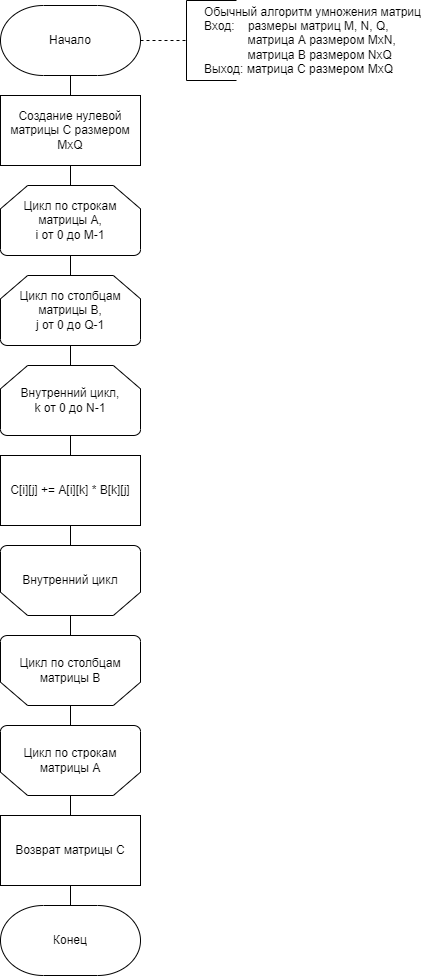
\includegraphics[scale=0.72]{simple.png}}
\caption*{Рисунок 2.1~--- Стандартный алгоритм умножения матриц}
\end{figure}

\begin{figure}[H]
\center{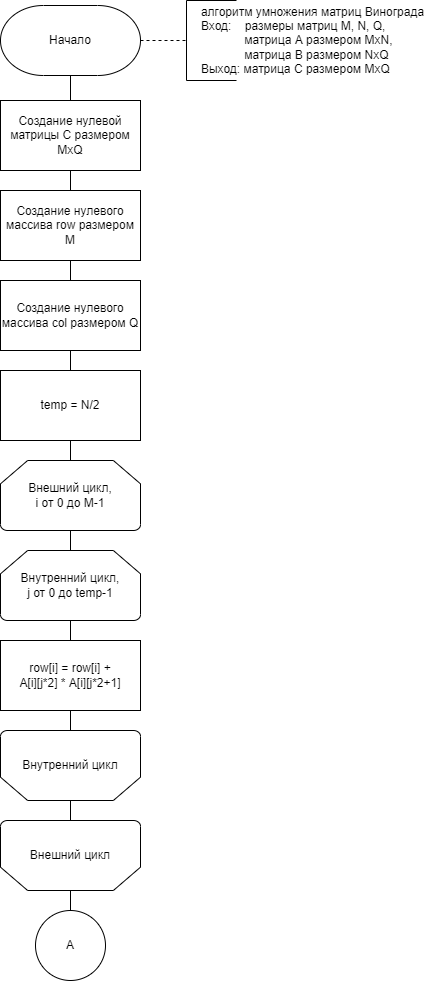
\includegraphics[scale=0.72]{vin1.png}}
\end{figure}

\begin{figure}[H]
\center{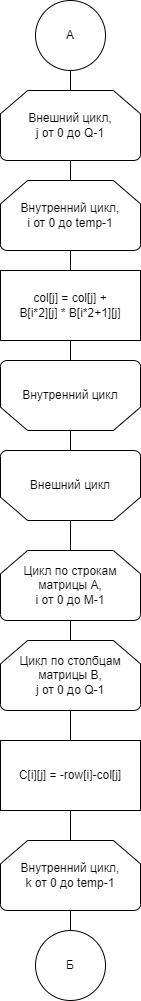
\includegraphics[scale=0.72]{vin2.png}}
\end{figure}

\begin{figure}[H]
\center{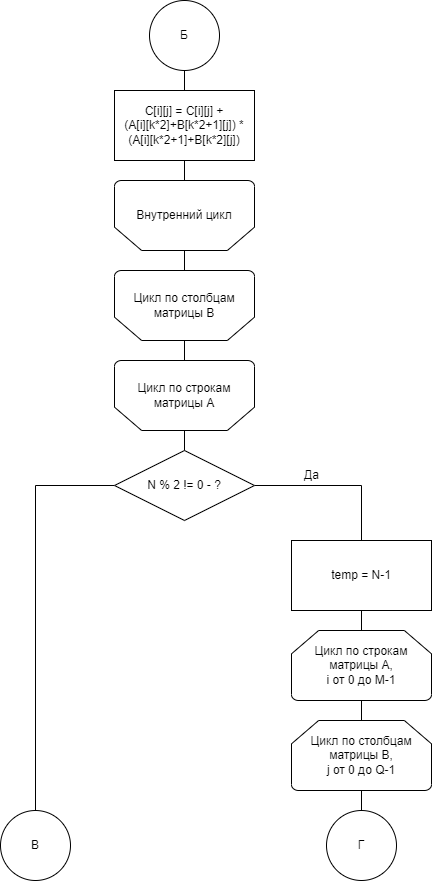
\includegraphics[scale=0.72]{vin3.png}}
\end{figure}

\begin{figure}[H]
\center{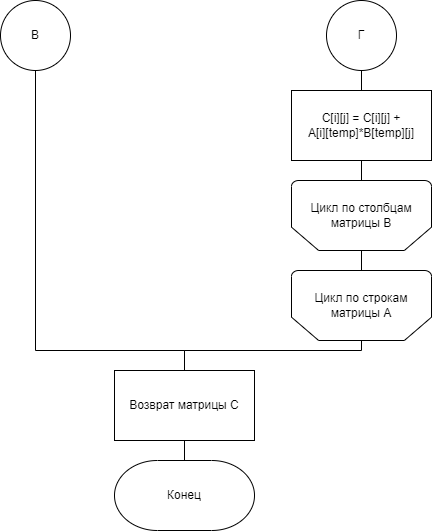
\includegraphics[scale=0.72]{vin4.png}}
\caption*{Рисунок 2.2~--- Алгоритм умножения матриц Копперсмита--Винограда}
\end{figure}

\begin{figure}[H]
\center{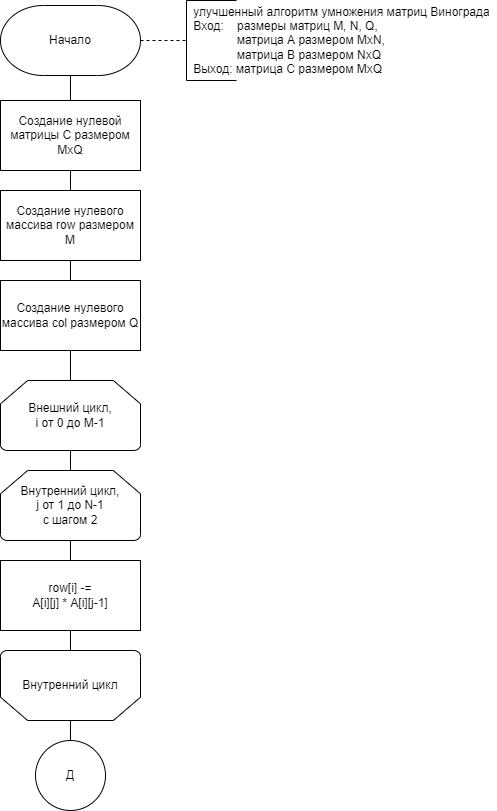
\includegraphics[scale=0.72]{optvin1.png}}
\end{figure}

\begin{figure}[H]
\center{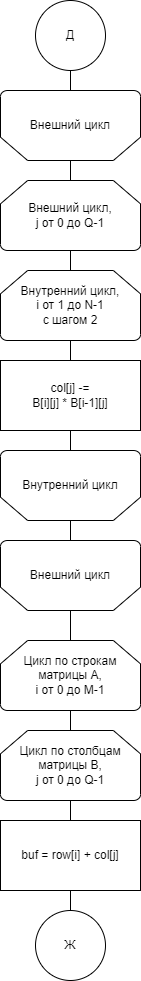
\includegraphics[scale=0.72]{optvin2.png}}
\end{figure}

\begin{figure}[H]
\center{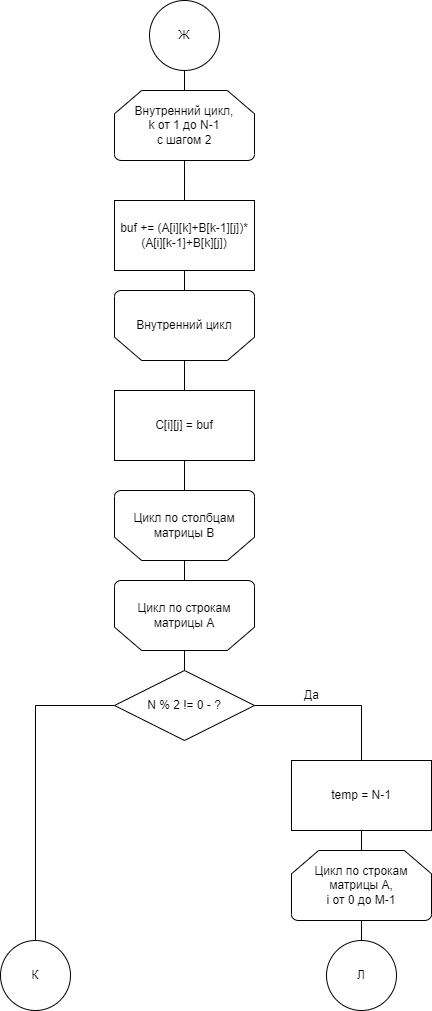
\includegraphics[scale=0.72]{optvin3.png}}
\end{figure}

\begin{figure}[H]
\center{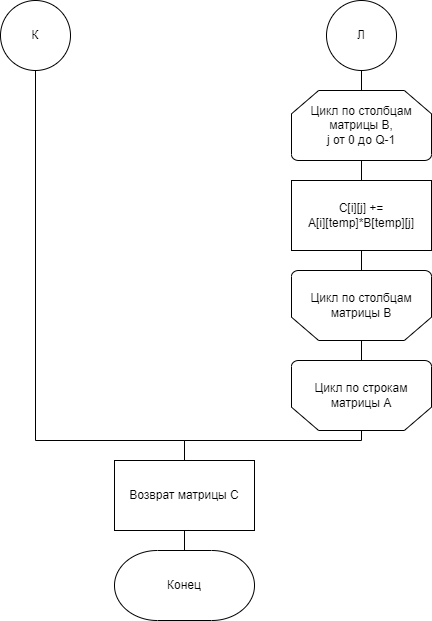
\includegraphics[scale=0.72]{optvin4.png}}
\caption*{Рисунок 2.3~--- Оптимизированный алгоритм умножения матриц Копперсмита--Винограда}
\end{figure}

\section*{2.2 Модель вычислений трудоемкости алгоритмов}
\addcontentsline{toc}{section}{2.2 Модель вычислений трудоемкости алгоритмов}

Будем использовать следующую модель вычислений трудоемкости алгоритмов:

\begin{enumerate}
	\item Трудоемкость базовых операций.
	
	Трудоемкость операций из списка (2.1) равна 2. $$ *, /, \%, *=, /= \eqno (2.1)$$Операции из списка (2.2) имеют трудоемкость 1.$$=, +, -, +=, -=, ==, !=, <, >, <=, >=, ||, \&, [] \eqno (2.2)$$
	\item Трудоемкость условного оператора.
	
	Трудоемкость условного перехода равна 0, а оператора if условие then A else B рассчитывается, как (2.3) в лучшем случае и как (2.4) в худщем случае.
	$$f_{\text{if}} = f_{\text{условия}} + min(f_{\text{A}}, f_{\text{B}})\eqno (2.3)$$	$$f_{\text{if}} = f_{\text{условия}} + max(f_{\text{A}}, f_{\text{B}})\eqno (2.4)$$ где $f_{\text{A}}, f_{\text{B}}$ ~--- трудоемкости блоков операций A и B соответственно.
	\item Трудоемкость цикла.
	
	Она рассчитывается, как (2.5).
	$$f_{\text{for}} = f_{\text{инициализации}} + f_{\text{условия}} + N(f_{\text{тела}} + f_{\text{инкремента}} + f_{\text{сравнения}})\eqno (2.5)$$
	\item Трудоемкость вызова функции равна 0.
\end{enumerate}

\section*{2.3 Трудоемкость алгоритмов умножения матриц}
\addcontentsline{toc}{section}{2.3 Трудоемкость алгоритмов умножения матриц}

Пусть размер матрицы $A$ во всех вычислениях обозначается как $M \times N$, а размер матрицы $B$~--- $N \times Q$. Трудоемкость создания результирующей матрицы будет опущена, поскольку эта операция одинакова для всех алгоритмов умножения матриц.

\subsection*{2.3.1 Стандартный алгоритм}
\addcontentsline{toc}{subsection}{2.3.1 Стандартный алгоритм}

Трудоёмкость стандартного алгоритма:
\begin{itemize}
	\item трудоёмкость цикла $i \in [0..M)$ : 
	$$f_i = 2 + M \cdot (2 + f_j) \eqno (2.6)$$
	
	\item трудоёмкость цикла $j \in[0..Q)$ :
	$$f_j = 2 + Q \cdot (2 + f_k) \eqno (2.7)$$
	
	\item трудоёмкость цикла $k \in[0..N)$ :
	$$f_k = 2 + N \cdot (2 + 12) \eqno (2.8)$$
\end{itemize}

Трудоёмкость стандартного алгоритма умножения матриц (2.9):

$$f_{simple} = 2 + M \cdot (2 + 2 + Q \cdot (2 + 2 + N \cdot (2 + 12))) =$$$$= 14MNQ + 4QM + 4M + 2 \approx 14QMN = O(QMN) \eqno (2.9)$$

\subsection*{2.3.2 Алгоритм Копперсмита--Винограда}
\addcontentsline{toc}{subsection}{2.3.2 Алгоритм Копперсмита--Винограда}

Трудоёмкость алгоритма Копперсмита--Винограда:
\begin{itemize}
	\item трудоемкость циклов инициализации векторов: 
	$$f_{initrow} = 2 + M \cdot (2 + 2 + \frac{N}{2} \cdot (2 + 15)), \eqno (2.10)$$
	$$f_{initcol} = 2 + Q \cdot (2 + 2 + \frac{N}{2} \cdot (2 + 15)), \eqno (2.11)$$
	\item трудоемкость цикла инициализации результирующей матрицы:
	$$f_{res} = 2 + M \cdot (2 + 2 + Q \cdot (2 + 7 + 2 + \frac{N}{2} \cdot (2 + 28))), \eqno (2.12)$$
	\item трудоемкость условного оператора:
	$$f_{if} = 3 + \left[ \begin{array}{cc}0, &\text{в лучшем случае}\\
\qquad 14MQ + 4M + 4, & \text{в худшем случае.}\end{array}\right. \eqno (2.13)$$
\end{itemize}

Трудоёмкость в \textbf{лучшем} случае (2.14).
$$f_{best} = 2 + M \cdot (2 + 2 + \frac{N}{2} \cdot (2 + 15)) +$$$$+ 2 + Q \cdot (2 + 2 + \frac{N}{2} \cdot (2 + 15)) + \eqno (2.14)$$$$+ 2 + M \cdot (2 + 2 + Q \cdot (2 + 7 + 2 + \frac{N}{2} \cdot (2 + 28))) + 3 =$$$$= 15MNQ + 11MQ + 8.5MN + 8.5NQ + 8M + 4Q + 9 \approx$$$$\approx
 15MNQ = O(MNQ)$$
 

Трудоёмкость в \textbf{худшем} случае (2.15).
$$f_{worst} = 15MNQ + 25MQ + 8.5MN + 8.5NQ + 12M + 4Q + 13 \approx$$$$\approx 15MNQ = O(MNQ) \eqno (2.15)$$

\subsection*{2.3.3 Оптимизированный алгоритм Копперсмита--Винограда}
\addcontentsline{toc}{subsection}{2.3.3 Оптимизированный алгоритм Копперсмита--Винограда}

Трудоёмкость оптимизированного алгоритма Копперсмита--Винограда:
\begin{itemize}
	\item трудоемкость циклов инициализации векторов: 
	$$f_{initrow} = 2 + M \cdot (2 + 2 + \frac{N}{2} \cdot (2 + 9)), \eqno (2.16)$$
	$$f_{initcol} = 2 + Q \cdot (2 + 2 + \frac{N}{2} \cdot (2 + 9)), \eqno (2.17)$$
	\item трудоемкость цикла инициализации результирующей матрицы:
	$$f_{res} = 2 + M \cdot (2 + 2 + Q \cdot (2 + 7 + 2 + \frac{N}{2} \cdot (2 + 15))), \eqno (2.18)$$
	\item трудоемкость условного оператора:
	$$f_{if} = 3 + \left[ \begin{array}{cc}0, &\text{в лучшем случае}\\
\qquad 11MQ + 4M + 4, & \text{в худшем случае.}\end{array}\right. \eqno (2.19)$$
\end{itemize}

Трудоёмкость в \textbf{лучшем} случае (2.20).
$$f_{best} = 2 + M \cdot (2 + 2 + \frac{N}{2} \cdot (2 + 9)) +$$$$+ 2 + Q \cdot (2 + 2 + \frac{N}{2} \cdot (2 + 9)) + \eqno (2.20)$$$$+ 2 + M \cdot (2 + 2 + Q \cdot (2 + 7 + 2 + \frac{N}{2} \cdot (2 + 15))) + 3 =$$$$= 8.5MNQ + 11MQ + 5.5MN + 5.5NQ + 8M + 4Q + 9 \approx$$$$\approx
8.5MNQ = O(MNQ)$$

Трудоёмкость в \textbf{худшем} случае (2.21).
$$f_{worst} = 8.5MNQ + 22MQ + 5.5MN + 5.5NQ + 12M + 4Q + 13 \approx$$$$\approx 8.5MNQ = O(MNQ) \eqno (2.21)$$

\section*{2.4 Вывод по конструкторской части}
\addcontentsline{toc}{section}{2.4 Вывод по конструкторской части}

На основе теоретических данных, полученных из аналитического раздела, были построены схемы алгоритмов умножения матриц. Оценены их трудоемкости.

При умножении матриц трудоемкость будет зависеть от размеров матриц в каждом конкретном случае. Из расчетов видно, что оптимизация алгоритма Копперсмита--Винограда позволила достичь меньшей трудоемкости в сравнении со стандартным алгоритмом.

\chapter*{3 Технологическая часть}
\addcontentsline{toc}{chapter}{3 Технологическая часть}

В данном разделе приведены средства реализации и листинги кода.

\section*{3.1 Требования к ПО}
\addcontentsline{toc}{section}{3.1 Требования к ПО}

К программе предъявляется ряд требований:
\begin{itemize}
	\item на вход ПО получает размеры двух матриц, а также сами элементы матриц;
	\item на выходе~--- результирующая матрица, полученная путем умножения двух исходных.
\end{itemize}

\section*{3.2 Средства реализации}
\addcontentsline{toc}{section}{3.2 Средства реализации}

Для реализации ПО был выбран язык программирования \verb|Python| [1]. Это обусловлено знанием возможностей языка, что обеспечит высокую скорость написания программы без потери ее качества. 

В качестве среды разработки выбрана \verb|Visual Studio Code| [3]. Удобства написания кода и его автодополнения стали ключевыми при выборе.

\section*{3.3 Реализация алгоритмов}
\addcontentsline{toc}{section}{3.3 Реализация алгоритмов}

В листингах 3.1 - 3.3 приведены реализации трёх алгоритмов умножения матриц.

\newpage
\begin{lstlisting}[title=Листинг 3.1~--- Алгоритм Копперсмита--Винограда]
def dotMatrixVinograd(a, b):
	if (len(b) != len(a[0])):
		raise ValueError

	m = len(a)
	n = len(a[0])
	q = len(b[0])
	c = [[0] * q for i in range(m)]

	row = [0] * m
	col = [0] * q

	temp = n // 2
	for i in range(m):
		for j in range(temp):
			row[i] = row[i] + a[i][2*j] * a[i][2*j + 1]

	for j in range(q):
		for i in range(temp):
			col[j] = col[j] + b[2*i][j] * b[2*i + 1][j]

	for i in range(m):
		for j in range(q):
			c[i][j] = -row[i] - col[j]
			for k in range(temp):
				c[i][j] = c[i][j] + (a[i][2*k+1] + b[2*k][j]) * (a[i][2*k] + b[2*k+1][j])

	if n % 2:
		temp = n - 1
		for i in range(m):
			for j in range(q):
				c[i][j] = c[i][j] + a[i][temp] * b[temp][j]

	return c
\end{lstlisting}

\newpage
\begin{lstlisting}[title=Листинг 3.2~--- Оптимизированный алгоритм Копперсмита--Винограда]
def dotMatrixVinogradOpt(a, b):
	if (len(b) != len(a[0])):
		raise ValueError

	m = len(a)
	n = len(a[0])
	q = len(b[0])
	c = [[0] * q for i in range(m)]

	row = [0] * m
	col = [0] * q

	for i in range(m):
		for j in range(1, n, 2):
			row[i] -= a[i][j] * a[i][j - 1]

	for j in range(q):
		for i in range(1, n, 2):
			col[j] -= b[i][j] * b[i - 1][j]

	for i in range(m):
		for j in range(q):
			buf = row[i] + col[j]
			for k in range(1, n, 2):
				buf += (a[i][k - 1] + b[k][j]) * (a[i][k] + b[k-1][j])
			c[i][j] = buf

	if n % 2:
		temp = n - 1
		for i in range(m):
			for j in range(q):
				c[i][j] += a[i][temp] * b[temp][j]

	return c
\end{lstlisting}

\newpage
\begin{lstlisting}[title=Листинг 3.3~--- Стандартный алгоритм умножения матриц]
def dotMatrix(a, b):
	if (len(b) != len(a[0])):
		raise ValueError

	m = len(a)
	n = len(a[0])
	q = len(b[0])
	c = [[0] * q for i in range(m)]

	for i in range(m):
		for j in range(q):
			for k in range(n):
				c[i][j] = c[i][j] + a[i][k] * b[k][j]

	return c
\end{lstlisting}

\section*{3.4 Тестовые данные}
\addcontentsline{toc}{section}{3.4 Тестовые данные}

В таблице (3.1) приведены тесты для функций, реализующих алгоритмы умножения матриц.

\begin{table}[h]
	\caption*{Таблица 3.1~--- Тестирование функций}
		\begin{tabular}[l]{|c|c|c|}
			\hline
			Входные матрицы & Результат & Ожидаемый результат \\ 
			\hline
			$\begin{pmatrix}
			2 & 1\\
			3 & 3\\
			-1 & 2
			\end{pmatrix} \times \begin{pmatrix}
			-5 & 1\\
			3 & -2
			\end{pmatrix}$ & $\begin{pmatrix}
			-7 & 0\\
			-6 & -3\\
			11 & -5
			\end{pmatrix}$  & $\begin{pmatrix}
			-7 & 0\\
			-6 & -3\\
			11 & -5
			\end{pmatrix}$\\\hline
			$\begin{pmatrix}
			1 & 2 & 3\\
			1 & 2 & 3\\
			1 & 2 & 3
			\end{pmatrix} \times \begin{pmatrix}
			1 & 2 & 3\\
			1 & 2 & 3\\
			1 & 2 & 3
			\end{pmatrix}$  & $\begin{pmatrix}
			6 & 12 & 18\\
			6 & 12 & 18\\
			6 & 12 & 18
			\end{pmatrix}$ & $\begin{pmatrix}
			6 & 12 & 18\\
			6 & 12 & 18\\
			6 & 12 & 18
			\end{pmatrix}$\\\hline
			$\begin{pmatrix}
			-5 & 1 & 3
			\end{pmatrix} \times \begin{pmatrix}
			2\\
			-3\\
			6
			\end{pmatrix}$  & $\begin{pmatrix}
			5
			\end{pmatrix}$  & $\begin{pmatrix}
			5
			\end{pmatrix}$\\\hline
			$\begin{pmatrix}
			2\\
			-3\\
			6
			\end{pmatrix} \times \begin{pmatrix}
			-5 & 1 & 3
			\end{pmatrix}$  & $\begin{pmatrix}
			-10 & 2 & 6\\
			15 & -3 & -9\\
			-30 & 6 & 18
			\end{pmatrix}$  & $\begin{pmatrix}
			-10 & 2 & 6\\
			15 & -3 & -9\\
			-30 & 6 & 18
			\end{pmatrix}$\\\hline
			$\begin{pmatrix}
			6
			\end{pmatrix} \times \begin{pmatrix}
			-5
			\end{pmatrix}$  & $\begin{pmatrix}
			-30
			\end{pmatrix}$  & $\begin{pmatrix}
			-30
			\end{pmatrix}$\\
			\hline
		\end{tabular}
\end{table}

Все тесты пройдены успешно.

\section*{3.5 Вывод по технологической части}
\addcontentsline{toc}{section}{3.5 Вывод по технологической части}

В данном разделе были реализованы и протестированы алгоритмы умножения матриц: стандартный алгоритм, алгоритм Копперсмита--Винограда и оптимизированный алгоритм Копперсмита--Винограда.

\chapter*{4 Исследовательская часть}
\addcontentsline{toc}{chapter}{4 Исследовательская часть}

Исследуем быстродействие алгоритмов умножения матриц на практических тестах.

\section*{4.1 Технические характеристики}
\addcontentsline{toc}{section}{4.1 Технические характеристики}

Ниже приведены технические характеристики устройства, на котором было проведено тестирование ПО:

\begin{itemize}
	\item Операционная система Windows 10 64-разрядная.
	\item Оперативная память 16 ГБ.
	\item Процессор Intel(R) Core(TM) i5-4690 @ 3.50ГГц.
\end{itemize}

\section*{4.2 Время выполнения реализаций алгоритмов}
\addcontentsline{toc}{section}{4.2 Время выполнения реализаций алгоритмов}

Время выполнения реализаций алгоритмов замерялось с помощью специальной функции \verb|process_time()| [2] из модуля \verb|time|, которая возвращает значение в долях секунды процессорного времени текущего процесса. Контрольная точка возвращаемого значения не определена, поэтому допустима только разница между результатами последовательных вызовов.

На рисунках 4.1 - 4.4 показаны результаты работы ПО. Все значения отображены в секундах.

\begin{figure}[H]
	\center{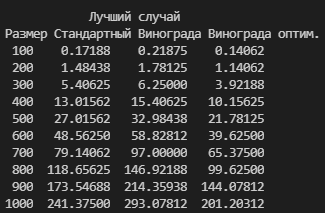
\includegraphics[scale=1.3]{1.png}}
	\caption*{Рисунок 4.1~--- Замеры на четных размерах матриц}
\end{figure}

\begin{figure}[H]
	\center{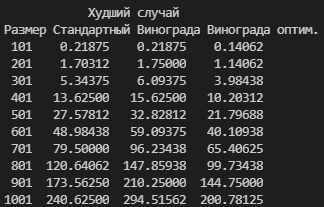
\includegraphics[scale=1.3]{2.png}}
	\caption*{Рисунок 4.2~--- Замеры на нечетных размерах матриц}
\end{figure}

\begin{figure}[H]
	\center{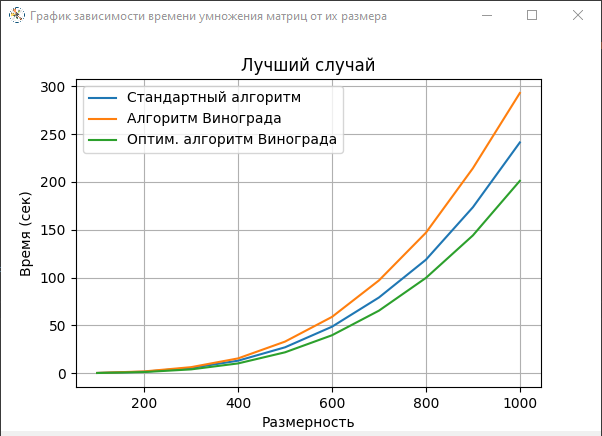
\includegraphics[scale=0.95]{3.png}}
	\caption*{Рисунок 4.3~--- Время выполнения реализаций алгоритмов на четных размерах матриц}
\end{figure}

\begin{figure}[H]
	\center{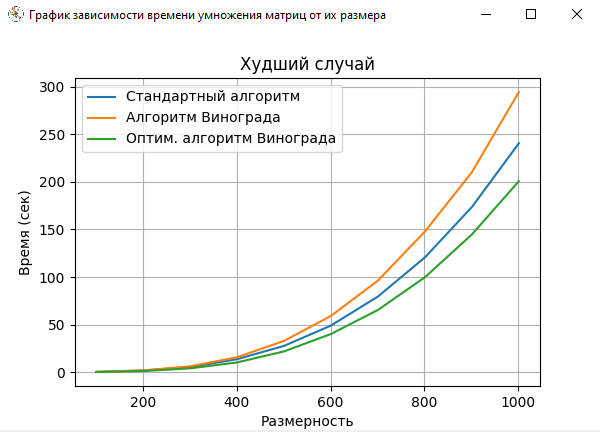
\includegraphics[scale=0.95]{4.png}}
	\caption*{Рисунок 4.4~--- Время выполнения реализаций алгоритмов на нечетных размерах матриц}
\end{figure}

\section*{4.3 Вывод по исследовательской части}
\addcontentsline{toc}{section}{4.3 Вывод по исследовательской части}

По результатам замеров самым быстрым алгоритмом оказался оптимизированный алгоритм Копперсмита--Винограда. При этом исходная версия алгоритма Копперсмита--Винограда уступает стандартному алгоритму умножения матриц как на четных, так и на нечетных размерностях матриц.


\chapter*{Заключение}
\addcontentsline{toc}{chapter}{Заключение}

В ходе проделанной работы была достигнута поставленная цель и решены следующие задачи:

\begin{itemize}
	\item были изучены алгоритмы умножения матриц: стандартный алгоритм, алгоритм Копперсмита--Винограда, оптимизированный алгоритм \newline Копперсмита--Винограда;
	\item был проведён сравнительный анализ трудоёмкости алгоритмов на основе теоретических расчетов и выбранной модели вычислений;
	\item эти алгоритмы были реализованы и успешно протестированы;
	\item был проведён сравнительный анализ алгоритмов на основе экспериментальных данных.
\end{itemize}

На основании анализа трудоемкости алгоритмов в выбранной модели вычислений было показано, что оптимизированный алгоритм Копперсмита--Винограда имеет меньшую трудоемкость. В среднем трудоемкость всех рассматриваемых алгоритмов имеет кубический характер зависимости от линейного размера матрицы. С помощью замеров времени выполнения реализаций алгоритмов умножения матриц была доказана посчитанная теоретически трудоемкость алгоримов. Таким образом, оптимизированный алгоритм Копперсмита--Винограда работает быстрее остальных рассматриваемых алгоритмов умножения матриц, при этом его исходная версия работает медленнее стандартного алгоритма.

\chapter*{Литература}
\addcontentsline{toc}{chapter}{Литература}

[1] Python [Электронный ресурс]. Режим доступа: https://python.org. Дата обращения: 22.10.2021.\\

[2] Модуль time [Электронный ресурс]. Режим доступа: \newline https://docs.python.org/3/library/time.html. Дата обращения: 22.10.2021.\\

[3] Visual Studio Code - Code Editing [Электронный ресурс]. Режим доступа: https://code.visualstudio.com. Дата обращения: 22.10.2021.\\

[4] Coppersmith D., Winograd S. 1990, Matrix multiplication via arithmetic Progressions, J. Symbolic Computation., Т. 9, Изд. 3, С. 251-280.

\end{document}